\chapter{K"unstliche neuronale Netze (unfinished)}
{
- Ablauf: Training, Testing, Using?\\
- k"unstliche Intelligenz und Maschinen lernen\\
- Was k"onnen sie: label und prediction\\
http://deeplearning4j.org/neuralnet-overview\\
Neural networks are a set of algorithms, modeled loosely after the human brain, that are designed to recognize patterns. They interpret sensory data through a kind of machine perception, labeling or clustering raw input. The patterns they recognize are numerical, contained in vectors, into which all real-world data, be it images, sound, text or time series, must be translated.
They help group unlabeled data according by similarities among the example inputs, and they classify data when they have a labeled dataset to train on. To be more precise, neural networks extract features that are fed to other algorithms for clustering and classification.

\section{Feedforward Netzwerke (unfinished)}
Ein Feedforward Netzwerk besteht aus Layern und Neuronen. Die Neuronen sind f"ur die Berechnungen zust"andig w"ahrend die Layer den Aufbau des Netzes bestimmen. Abbildung 2.1 zeigt einen m"oglichen Aufbau eines k"unstliches Neurons.
\renewcommand{\figurename}{Abb.}
\begin{figure}[htp]
\centering
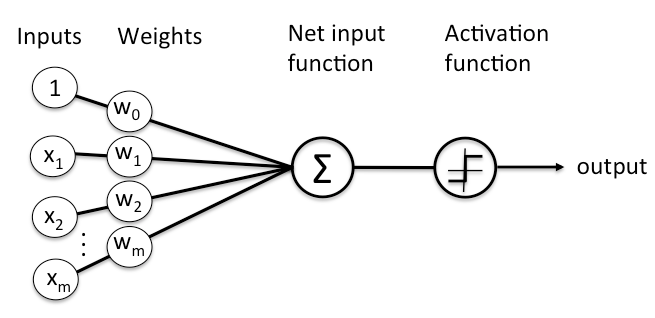
\includegraphics[width=0.60\textwidth]{pictures/perceptron_node.png}
\caption[Feedforward Neuron]{m"ogliches Aussehen eines Feedforward Neurons (Quelle: \cite{FNeuron})}
\end{figure}
Dieses Neuron besteht aus 1 bis x\textsubscript{m} Eing"angen (Inputs) mit Gewichten (Weights), einer Input Funktion (Net input function), einer Aktivierungsfunktion (Activation function) und einem Ausgang (Outputs). Die zu verarbeiteten Daten werden an die Eing"ange gelegt, durch die zugeh"origen Gewichte verst"arkt oder abgeschw"acht und anschlie{\ss}end aufsummiert. Die entstandene Summe wird dann an die Aktivierungsfunktion "ubergeben, welche das Ergebnis dieses Neurons festlegt.

Ein Layer besteht aus einer Reihe von Neuronen beliebiger Anzahl. Ein k"unstliches neuronales Netz setze sich aus einem Input Layer, einem Output Layer und beliebig vielen Hidden Layern zusammen. Hat ein Netz mehr als ein Hidden Layer so wird es auch als Deep Learning Netz bezeichnet.
\renewcommand{\figurename}{Abb.}
\begin{figure}[htp]
\centering
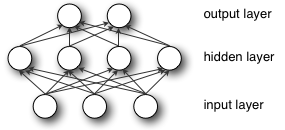
\includegraphics[width=0.50\textwidth]{pictures/mlp.png}
\caption[Aufbau eines Feedforward Netzes]{Aufbau eines Feedforward Netzes (Quelle: \cite{FNet})} 
\end{figure}
Abbildung 2.2 zeigt ein Feedforward Netzwerk. Bei diesem Netz besitzt das Input Layer drei Neuronen, das Hidden Layer hat vier und das Output Layer hat zwei Neuronen. Die Ergebnisse des Input und Hidden Layers dienen dem nachfolgenden Layer als Eingang.

Ein neuronales Netz kann anhand von Trainingsdaten eine Funktion erlernen, indem es die Gewichte ver"andert. Da bei Trainingsdaten das Ergebnis bekannt ist, muss das Netz die Gewichte so bestimmen, dass sie mit den Eingangsdaten den gew"unschten Ausgang mit m"oglichst kleinem Fehler abbilden. Das Ziel ist m"oglichst schnell den Punkt zu erreichen an dem der Fehler am kleinsten ist. Um dies zu erreichen wiederholt das Netz die folgenden Schritte: Ergebnis anhand der aktuellen Gewichte bestimmen, Fehler messen, Gewichte aktuallisieren.
Eine weitverbreitete Optimierungsfunktions zur Gewichtebestimmung hei{\ss}t Gradient Descent. Sie beschreibt das Verh"altnis des Fehlers zu einem einzelnen Gewicht und wie sich der Fehler ver"andert wenn das Gewicht angepasst wird.\\
Sources: - http://deeplearning4j.org/neuralnet-overview


\section{Recurrent Netzwerke (unfinished)}
Recurrent Neuronal Networks (RNN) betrachten im Gegensatz zu Feedforward Netzwerken nicht nur die aktuellen Eingangsdaten sondern auch die vorhergegangenen. Sie besitzen daher zwei Eingangsgr"o{\ss}en, n"amlich die gerade angelegten und die zur"uckgeleiteten aus dem vorherigen Zeitschritt.
\renewcommand{\figurename}{Abb.}
\begin{figure}[htp]
%%\begin{floatingfigure}[r]{textwidth}
\centering
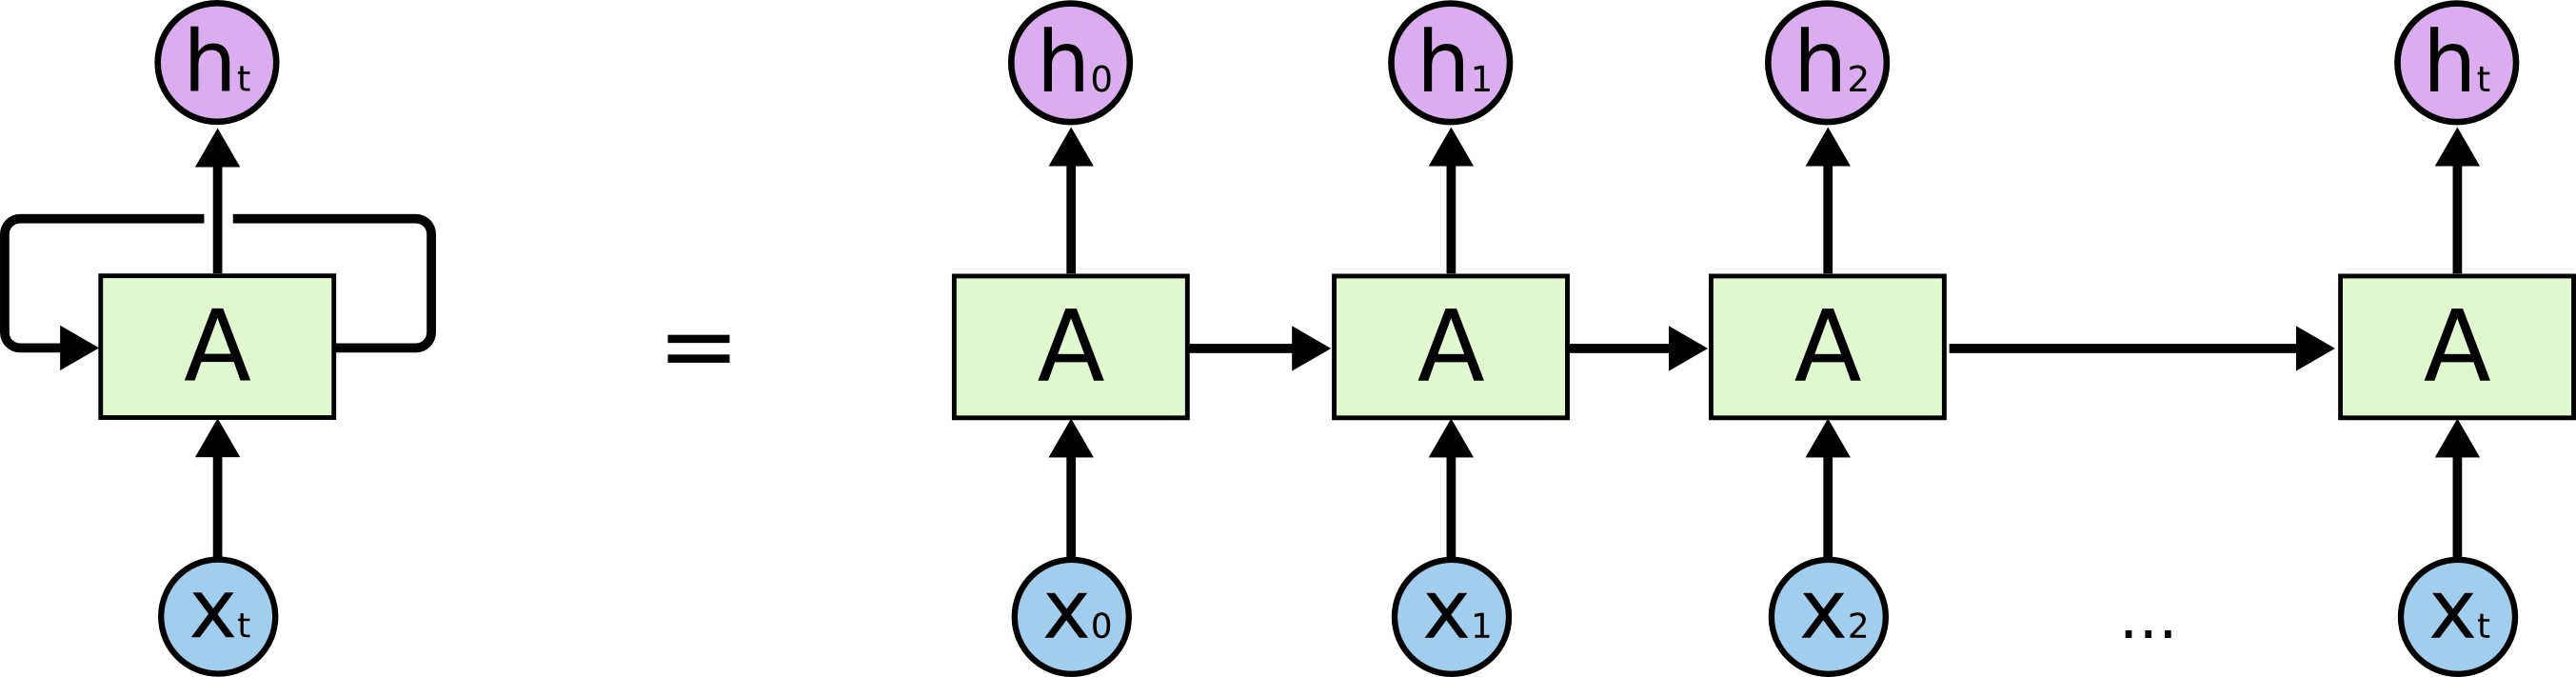
\includegraphics[width=0.60\textwidth]{pictures/RNN-unrolled.png}
\caption[RNN Neuron]{vereinfachte Darstellung eines RNN Neurons (Quelle: \cite{OlahImg})}
%%\end{floatingfigure} 
\end{figure}
Abbildung 2.3 zeigt links eine vereinfachte Darstellung eines RNN Neuron mit R"uckf"uhrung, aber ohne Gewichte oder Aktivierungsfunktion. Rechts ist das Ganze als zeitlicher Verlauf dargestellt. Im ersten Zeitschritt wird x\textsubscript{0} an den Eingang gelegt und h\textsubscript{0} als Ergebnis berechnet. Au{\ss}erdem f"uhrt ein Pfeil zum Neuron im zweiten Zeitschritt und dient dort als zweiter Eingang. Das Ergebnis, das ein Neuron liefert ist also immer vom vorherigen abh"angig. Man bezeichnet dies auch als Ged"achtnis des Netzes. Einem Netz ein Ged"achnis zu geben macht immer dann Sinn, wenn die Eingangsdaten eine Sequenz bilden und nicht komplett unabh"angig von einander sind. Im Gegensatz zu den Feedforward Netzen k"onnen Recurrent Netzwerke Sequenzen erfassen und sie zur Erzeugung ihrer Ausgaben nutzen. Dies ist zum Beispiel bei der automatischen Textgenerierung hilfreich, wo ein folgender Buchstabe immer vom vorherigen abh"angt und nicht willk"urlich gew"ahlt werden kann. Ein RNN ist in der Lage auf ein q ein u folgen zu lassen um sinnvolle W"orter zu bilden, ein Feedforward Netzwerk kann das nicht.\\
Sources:http://deeplearning4j.org/lstm.html, https://colah.github.io/posts/2015-08-Understanding-LSTMs/


\subsection{Backpropagation Through Time (unfinished)}
Um sinnvolle Ergebnisse von einem Netzwerk zu erhalten m"ussen die Gewichte solange angepasst werden, bis der Fehler am kleinsten ist. Dies wird mit Hilfe der Backpropagation gemacht, indem R"uckw"arts vom Fehler "uber die Ausg"ange, die Gewichte und die Eing"ange der verschiedenen Layer ein Zusammenhang zwischen Fehlergr"o{\ss}e und einzelnen Gewichtseinstellungen hergestellt wird. Durch die Backpropagation l"asst sich der Einfluss jedes Gewichtes auf den Fehler ermitteln und mit der Gradient Descent Methode der Fehler verringern.
Da bei Recurrent Netzen das Ergebnis und somit der Fehler nicht nur vom aktuellen Zeitschritt abh"angt, muss auch die Backpropagation erweitert werden um sinnvoll arbeiten zu k"onnen. Backpropagation Through Time (BPTT) erg"anzt die normale Backpropagation um den Faktor Zeit, so dass ein Einfluss auf den Fehler von einem Gewicht aus fr"uheren Schritten ermittelt werden kann. Abbildung 2.4 soll diesen Vorgang verdeutlichen. Sie zeigt ein Recurrent Netz das um drei Zeitschritte entrollt wurde indem Komponenten dupliziert wurden. Dadurch l"osen sich die R"uckf"uhrungen auf und das Netzwerk verh"alt sich wie ein Feedforward Netz. Der Einfluss jedes Gewichts kann nun anteilig berechnet und anschlie{\ss}end summiert werden, so dass ein einzelner Wert je Gewicht f"ur die Anpassung ermittelt wird.
\renewcommand{\figurename}{Abb.}
\begin{figure}[htp]
\centering
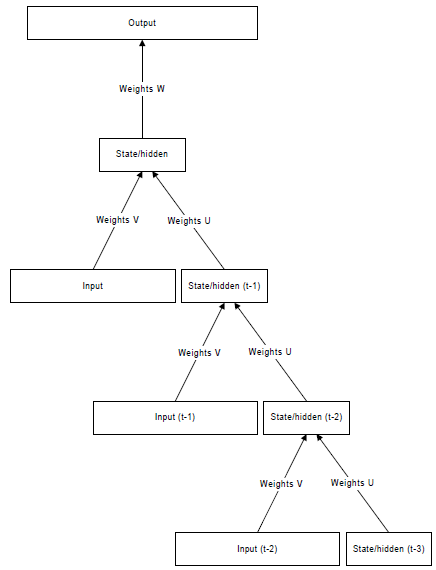
\includegraphics[width=0.8\textwidth]{pictures/bptt.png}
\caption[BPTT]{entrolltes RNN f"ur BPTT (Quelle: \cite{BPTT})}
\end{figure}
Dieses Verfahren ben"otigt nat"urlich mehr Speicher, da alle vorherigen Zust"ande und Daten f"ur eine bestimme Anzahl an Zeitschritten gespeichert werden m"ussen.\\
Sources: http://deeplearning4j.org/lstm.html,  10.1.1.16.6652.pdf


\subsection{Verschwindende und explodierende Gradienten (unfinished)}
Der Gradient stellt die Ver"anderung aller Gewichte in bezug auf Ver"anderung im Fehler dar. Wenn der Gradient unbekannt ist, ist eine Ver"anderung an den Gewichten zur Verkleinerung des Fehlers nicht m"oglich und das Netz ist nicht in der Lage zu lernen. Zu unbekannten Gradienten kann es kommen, da Informationen die durch ein Netz flie{\ss}en vielfach multipliziert werden. Multipliziert man einen Betrag regelm"a{\ss}ig mit einem Wert knapp gr"o{\ss}er Eins kann das Ergebnis unmessbar gro{\ss} werde und in diesem Fall spricht man von einem explodierenden Gradienten. Umgekehr f"uhrt eine widerholte Multiplikation eines Betrages mit einem Wert kleiner als Eins zu einem sehr kleinem Ergebnis. Der Wert kann so klein werden, dass er von einem Netz nicht mehr gelernt werden kann. Hier spricht man von einem verschwindenden Gradient.

Das Problem der explodierenden Gradienten l"asst sich durch eine sinnvolle Obergrenze beheben. Bei den verschwindenden Gradienten sieht eine L"osung wesentlich schwieriger aus.\\
Sources: http://deeplearning4j.org/lstm.html


\subsection{Problem der Langzeit-Abh"angigkeiten (unfinished)}
Wie bereits erw"ahnt sind RNNs in der Lage Sequenzen zu erkennen und mit Abh"angigkeiten zu arbeiten, doch diese F"ahigkeit ist leider begrenzt. Besteht nur eine kleine zeitliche L"ucke zwischen den von einander abh"angigen Daten, ist ein RNN in der Lage diesen Zusammenhang zu erkennen und die richtigen Schl"usse zu ziehen. Wird der zeitliche Abstand zwischen Eingabe der Daten und dem Zeitpunkt an dem sie f"ur ein Ergebnis ben"otigt werden jedoch sehr gro{\ss} kann ein RNN diesen Zusammenhang nicht mehr herstellen. Als Beispiel gibt \cite{Olah} in seinem Artikel ein Sprach-Model an, welches das n"achste Wort abh"angig vom Vorherigen vorhersagt. Ein RNN ist in der Lage im Satz {\glqq}Die Wolken sind im Himmel.{\grqq} das letzte Wort vorauszusagen, da der Abstand von Himmel und Wolken sehr klein ist. Im Text {\glqq}Ich bin in Frankreich aufgewachsen. ... Ich spreche flie{\ss}end franz"osisch.{\grqq} kann der Abstand zum letzten Wort aber sehr gro{\ss} sein und die vorherigen W"orter lassen lediglich den Schluss zu das eine Sprache folgen muss. Denn Kontext, dass es sich sehr wahrscheinlich um franz"osisch handelt, erh"allt man nur durch den ersten Satz. Ein RNN kann sich aber keinen ganzen Text merken und somit hier den Zusammenhang von Frankreich und franz"osisch nicht lernen.

Um das Problem der Langzeit-Abh"angigkeiten zu l"osen, benutzt man LSTMs.\\
Sources: https://colah.github.io/posts/2015-08-Understanding-LSTMs/


\section{Long Short-Term Memory (LSTM) (unfinished)}
LSTMs are explicitly designed to avoid the long-term dependency problem. Remembering information for long periods of time is practically their default behavior, not something they struggle to learn!

Long Short-Term Memory (LSTM) Netze sind eine besondere Art von Recurrent Netzwerken, die mit Langzeit-Abh"angigkeiten arbeiten k"onnen. Sie bestehen aus Speicherzellen, in die Informationen geschrieben und wieder herausgelesen werden k"onnen. Mit Hilfe von Toren (Gates), die ge"offnet oder geschlossen werden, entscheidet eine Zelle was gespeichert wird und wann ein Auslesen, Reinschreiben und L"oschen erlaubt ist. Diese Tore sind analog und durch eine Sigmoid-Funktion implementiert, so dass sich ein Bereich von 0 bis 1 ergibt. (Analog hat den Vorteil gegen"uber digital dass es differenzierbar ist und somit f"ur die Backpropagation geeignet.) Genau wie die Eing"ange bei den Feedforward und Recurrent Netzen besitzen die Tore Gewichte. Diese Gewichte werden ebenfalls w"ahrend des Lernprozesses angepasst, so dass die Zelle lernt wann Daten eingelassen, ausgelesen oder gel"oscht werden.
\renewcommand{\figurename}{Abb.}
\begin{figure}[h]
\centering
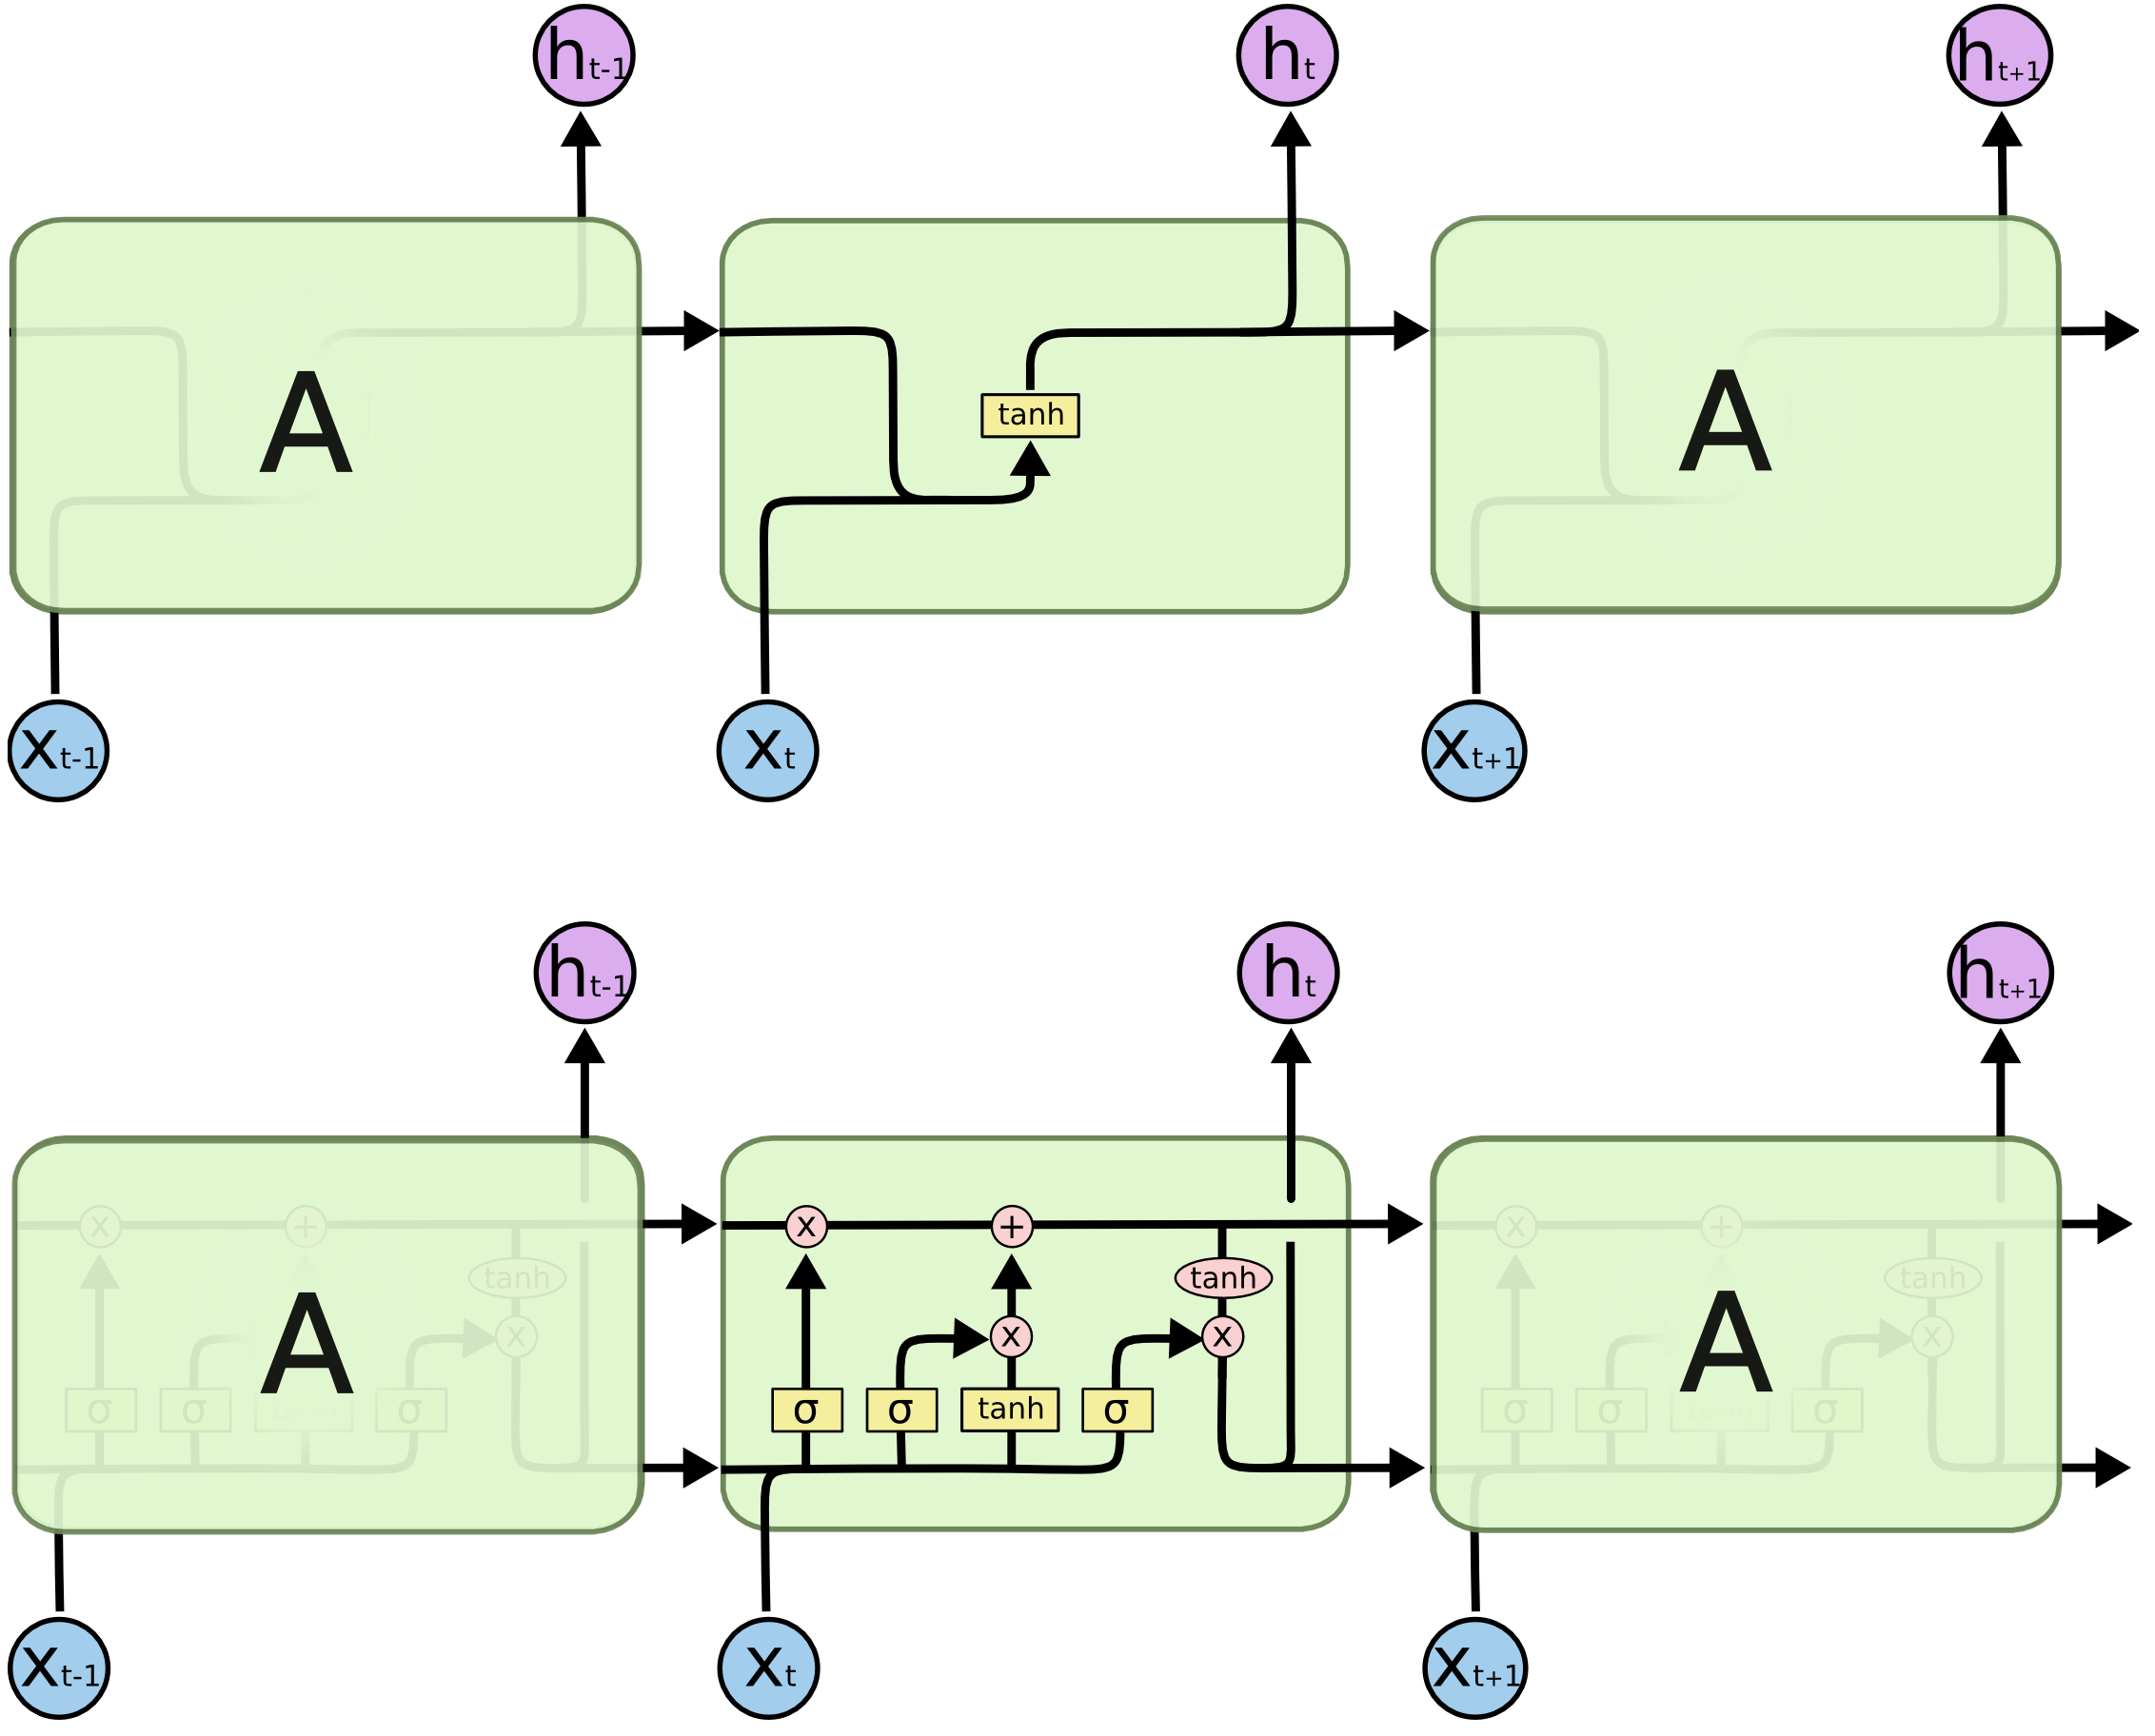
\includegraphics[width=1\textwidth]{pictures/SRN-LSTM-chain.png}
\caption[Vergleich RNN und LSTM]{Vergleich RNN und LSTM (Quelle: \cite{OlahImg})}
\end{figure}

Abbildung 2.5 zeigt zum Vergleich oben ein simples Recurrent Netz und unten ein LSTM Netz. Beide sind "uber drei Zeitschritte dargestellt. 
...
All recurrent neural networks have the form of a chain of repeating modules of neural network. In standard RNNs, this repeating module will have a very simple structure, such as a single tanh layer.
LSTMs also have this chain like structure, but the repeating module has a different structure. Instead of having a single neural network layer, there are four, interacting in a very special way.
In the above diagram, each line carries an entire vector, from the output of one node to the inputs of others. The pink circles represent pointwise operations, like vector addition, while the yellow boxes are learned neural network layers.
\\Sources: https://colah.github.io/posts/2015-08-Understanding-LSTMs/, http://deeplearning4j.org/lstm.html

LSTMs help preserve the error that can be backpropagated through time and layers. By maintaining a more constant error, they allow recurrent nets to continue to learn over many time steps (over 1000), thereby opening a channel to link causes and effects remotely.

You may wonder why LSTMs have a forget gate when their purpose is to link distant occurrences to a final output. Well, sometimes it’s good to forget. If you’re analyzing a text corpus and come to the end of a document, for example, you may have no reason to believe that the next document has any relationship to it whatsoever, and therefore the memory cell should be set to zero before the net ingests the first element of the next document.


Further links: (could be sources for pictures)\\
http://people.idsia.ch/~juergen/rnn.html\\
https://karpathy.github.io/2015/05/21/rnn-effectiveness/\\
https://www.cs.cmu.edu/~bhiksha/courses/deeplearning/Fall.2015/pdfs/Werbos.backprop.pdf\\
http://www.cs.toronto.edu/~graves/phd.pdf\\
http://www.felixgers.de/papers/phd.pdf\\
http://arxiv.org/pdf/1503.04069.pdf\\


\subsection{Bauteile einer Speicherzelle}
\subsubsection{Zellzustand}
The key to LSTMs is the cell state, the horizontal line running through the top of the diagram.
The cell state is kind of like a conveyor belt. It runs straight down the entire chain, with only some minor linear interactions. It’s very easy for information to just flow along it unchanged.
\renewcommand{\figurename}{Abb.}
\begin{figure}[htp]
\centering
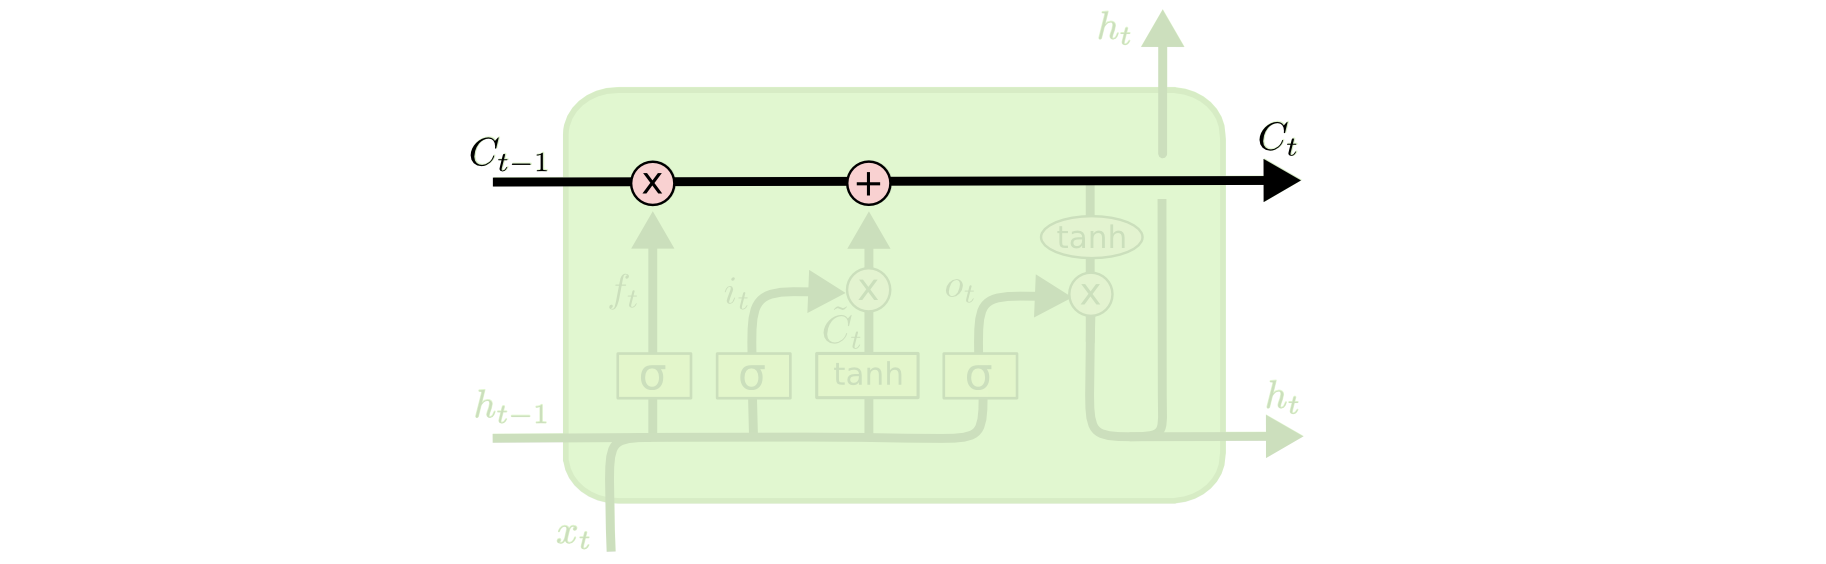
\includegraphics[width=0.60\textwidth]{pictures/LSTM3-C-line.png}
\caption[LSTM C line]{LSTM C line (Quelle: \cite{OlahImg})}
\end{figure}
The LSTM does have the ability to remove or add information to the cell state, carefully regulated by structures called gates.
Gates are a way to optionally let information through. They are composed out of a sigmoid neural net layer and a pointwise multiplication operation.
The sigmoid layer outputs numbers between zero and one, describing how much of each component should be let through. A value of zero means "let nothing through," while a value of one means "let everything through!"
An LSTM has three of these gates, to protect and control the cell state.

\subsubsection{Forget Gate}
The first step in our LSTM is to decide what information we’re going to throw away from the cell state. This decision is made by a sigmoid layer called the "forget gate layer." It looks at ht−1 and xt, and outputs a number between 0 and 1 for each number in the cell state Ct−1. A 1 represents "completely keep this" while a 0 represents "completely get rid of this."
\renewcommand{\figurename}{Abb.}
\begin{figure}[htp]
\centering
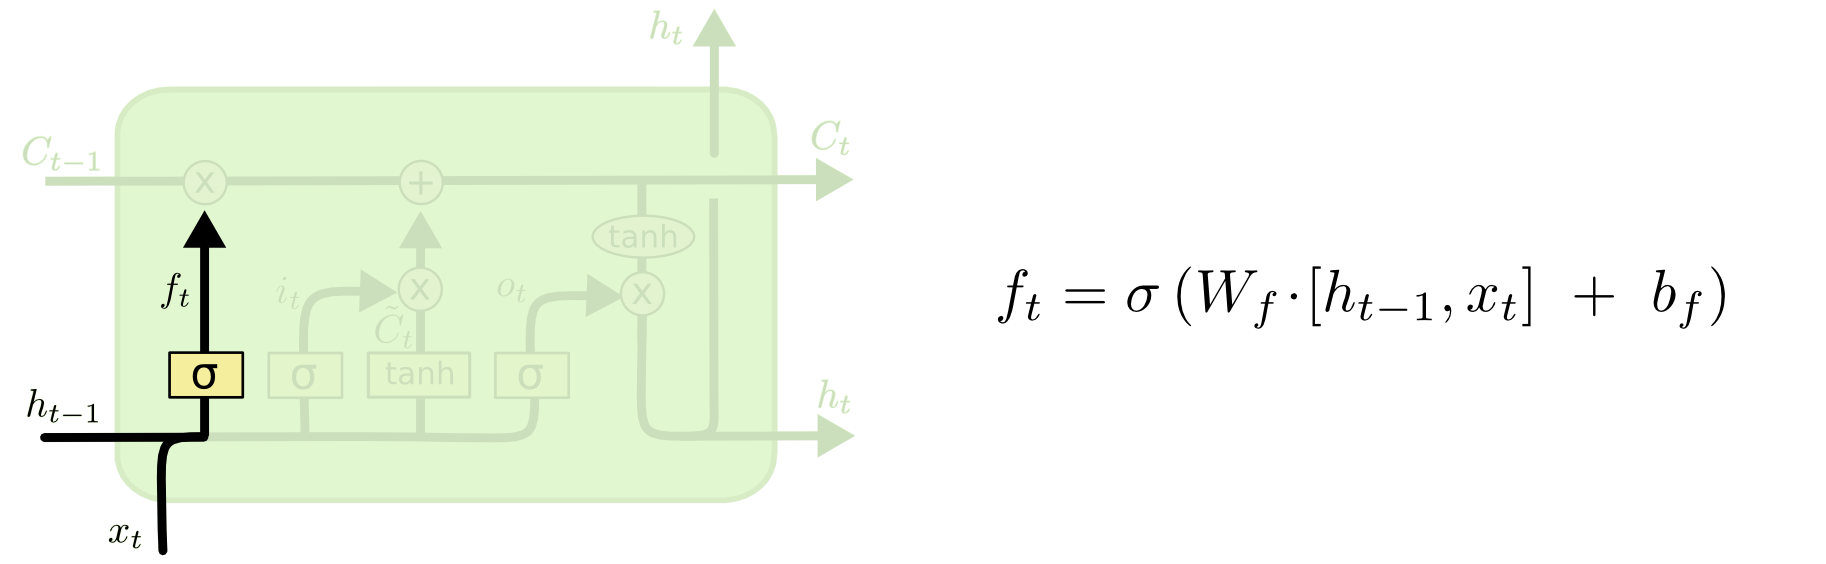
\includegraphics[width=0.60\textwidth]{pictures/LSTM3-focus-f.png}
\caption[LSTM focus f]{LSTM focus f (Quelle: \cite{OlahImg})}
\end{figure}

\subsubsection{Input gate}
The next step is to decide what new information we’re going to store in the cell state. This has two parts. First, a sigmoid layer called the "input gate layer" decides which values we’ll update. Next, a tanh layer creates a vector of new candidate values, C~t, that could be added to the state. In the next step, we’ll combine these two to create an update to the state.
\renewcommand{\figurename}{Abb.}
\begin{figure}[htp]
\centering
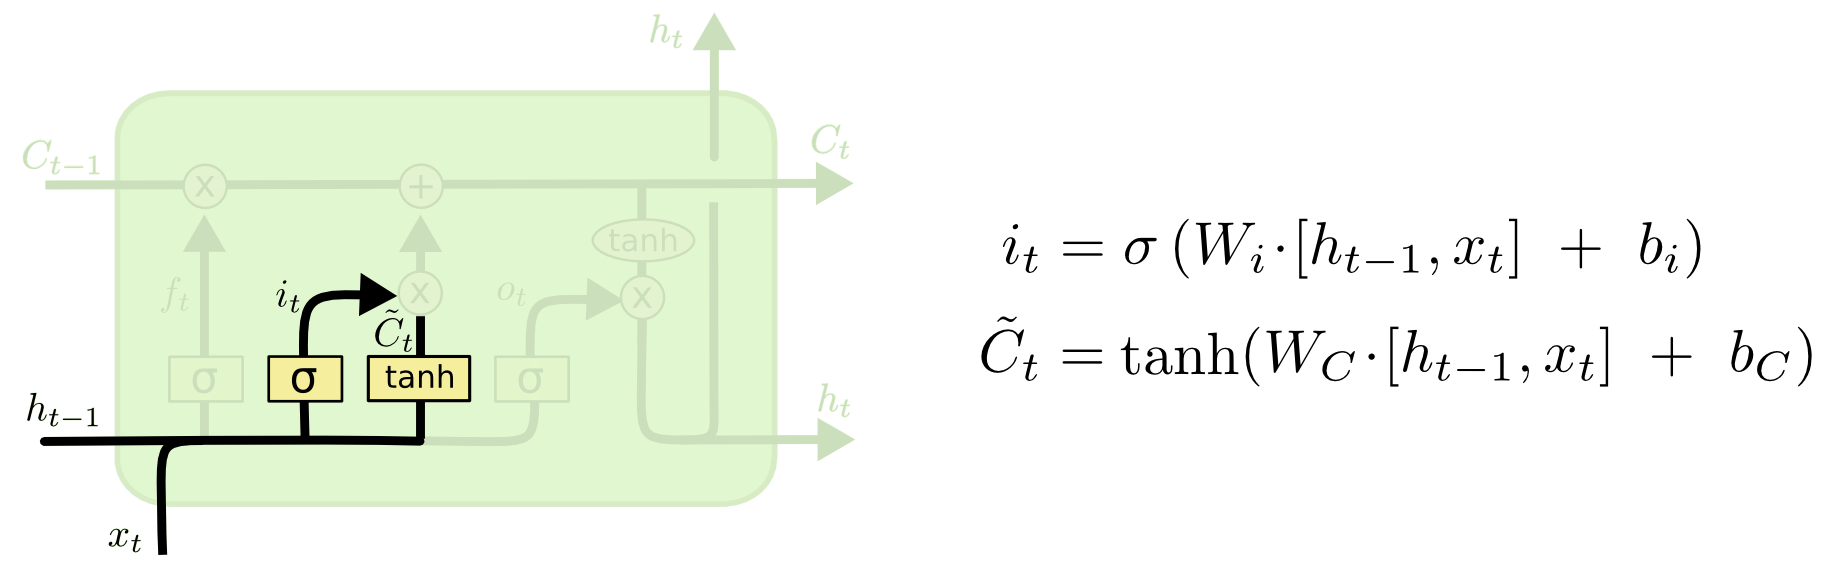
\includegraphics[width=0.60\textwidth]{pictures/LSTM3-focus-i.png}
\caption[LSTM focus i]{LSTM focus i (Quelle: \cite{OlahImg})}
\end{figure}

\subsubsection{Update Cell state}
It’s now time to update the old cell state, Ct−1, into the new cell state Ct. The previous steps already decided what to do, we just need to actually do it.
We multiply the old state by ft, forgetting the things we decided to forget earlier. Then we add it∗C~t. This is the new candidate values, scaled by how much we decided to update each state value.
\renewcommand{\figurename}{Abb.}
\begin{figure}[htp]
\centering
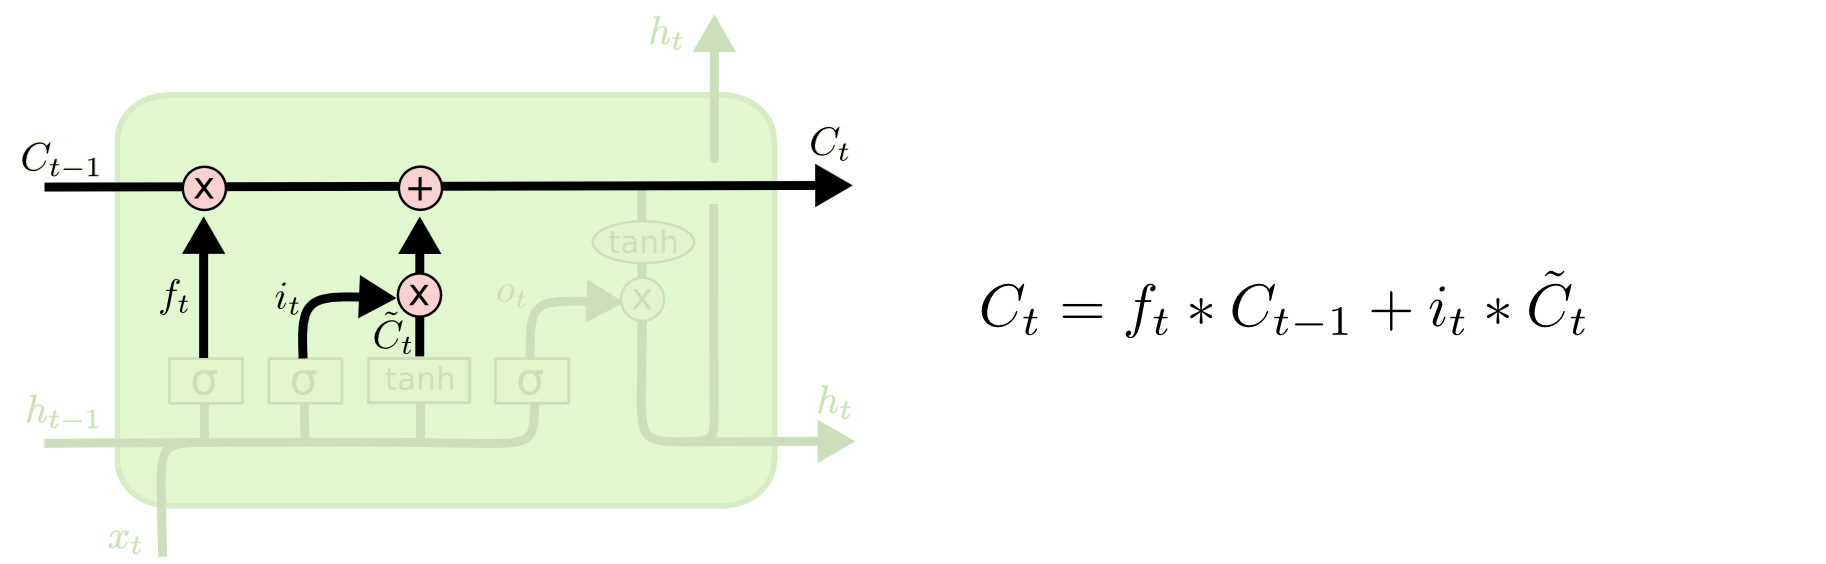
\includegraphics[width=0.60\textwidth]{pictures/LSTM3-focus-C.png}
\caption[LSTM focus C]{LSTM focus C (Quelle: \cite{OlahImg})}
\end{figure}

\subsubsection{Output}
Finally, we need to decide what we’re going to output. This output will be based on our cell state, but will be a filtered version. First, we run a sigmoid layer which decides what parts of the cell state we’re going to output. Then, we put the cell state through tanh (to push the values to be between −1 and 1) and multiply it by the output of the sigmoid gate, so that we only output the parts we decided to.
\renewcommand{\figurename}{Abb.}
\begin{figure}[htp]
\centering
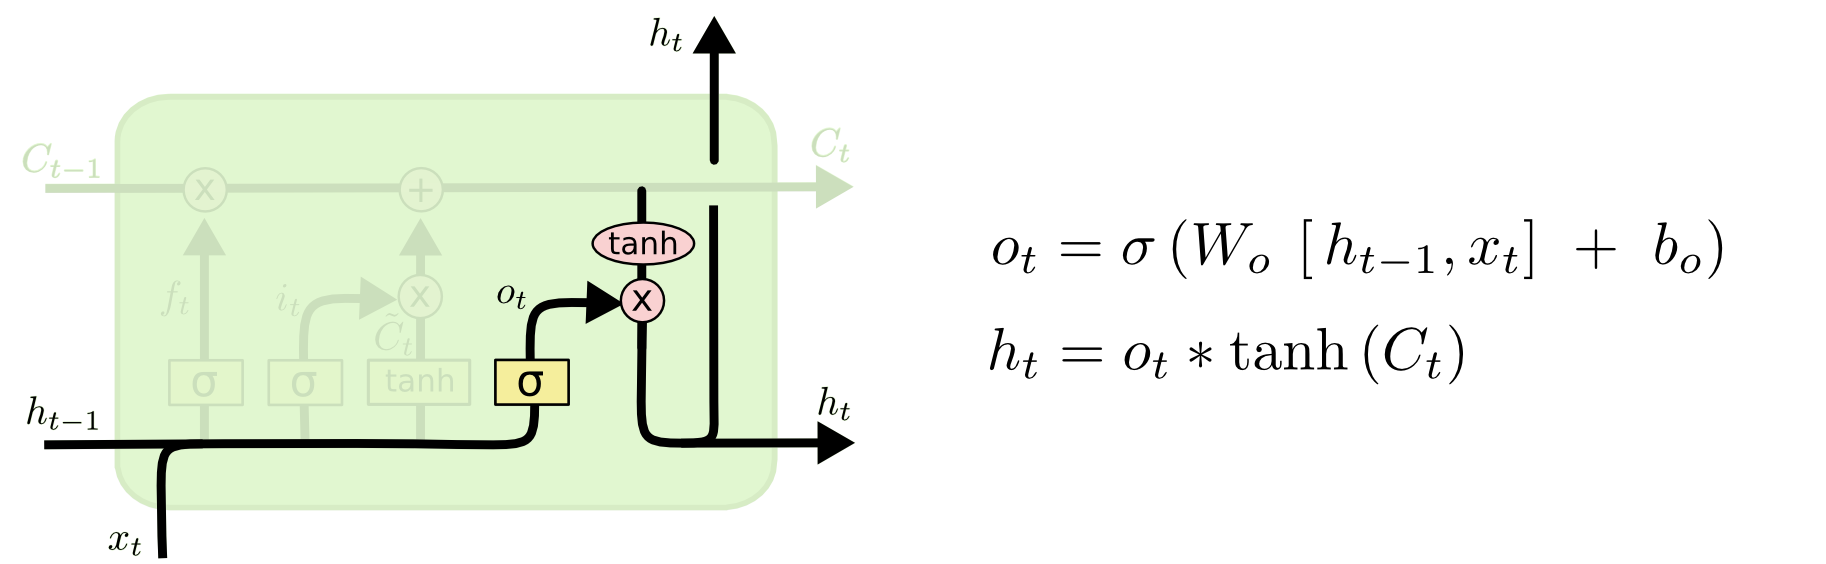
\includegraphics[width=0.60\textwidth]{pictures/LSTM3-focus-o.png}
\caption[LSTM focus o]{LSTM focus o (Quelle: \cite{OlahImg})} 
\end{figure}


\subsection{LSTM Varianten}
What I’ve described so far is a pretty normal LSTM. But not all LSTMs are the same as the above. In fact, it seems like almost every paper involving LSTMs uses a slightly different version. The differences are minor, but it’s worth mentioning some of them.

One popular LSTM variant, introduced by Gers \& Schmidhuber (2000), is adding "peephole connections." This means that we let the gate layers look at the cell state.
\renewcommand{\figurename}{Abb.}
\begin{figure}[htp]
\centering
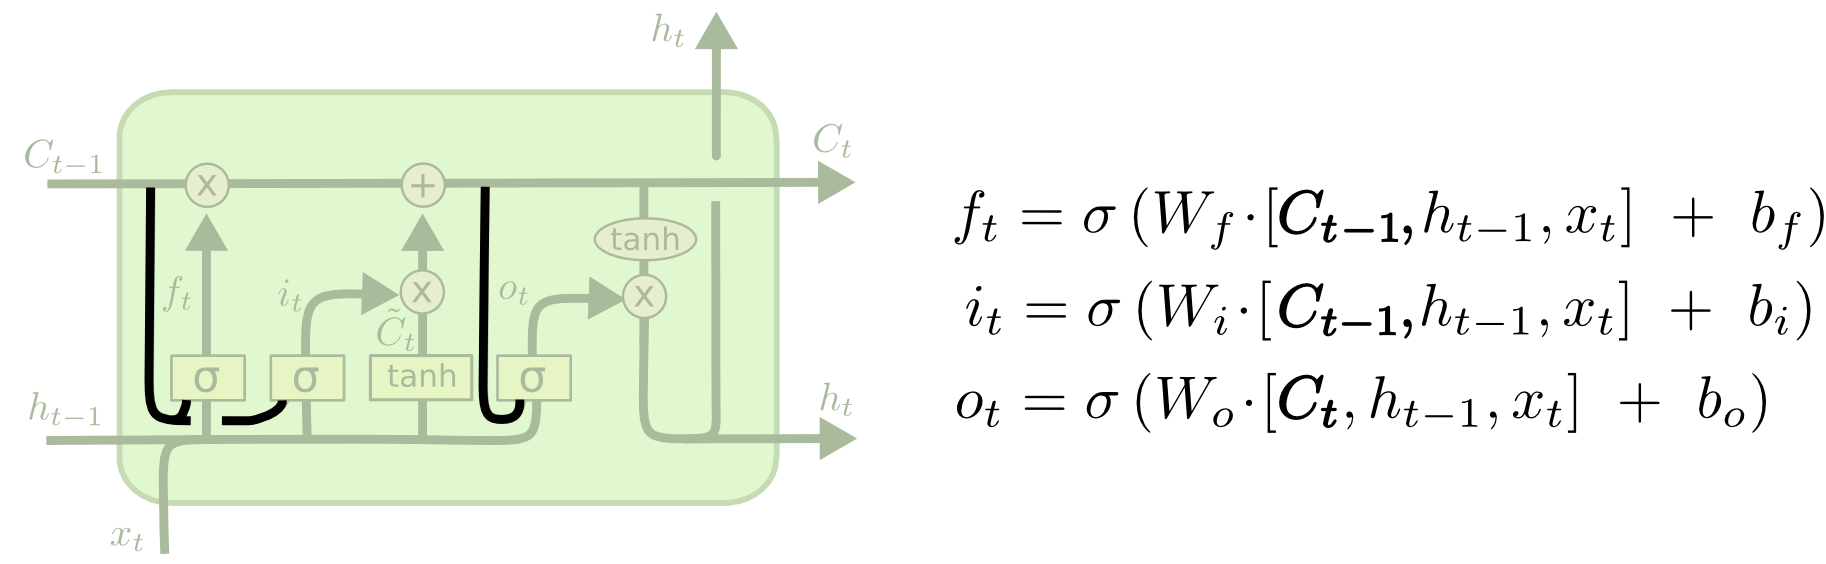
\includegraphics[width=0.60\textwidth]{pictures/LSTM3-var-peepholes.png}
\caption[LSTM peepholes]{LSTM peepholes (Quelle: \cite{OlahImg})}
\end{figure}
The above diagram adds peepholes to all the gates, but many papers will give some peepholes and not others.

Another variation is to use coupled forget and input gates. Instead of separately deciding what to forget and what we should add new information to, we make those decisions together. We only forget when we’re going to input something in its place. We only input new values to the state when we forget something older.
\renewcommand{\figurename}{Abb.}
\begin{figure}[htp]
\centering
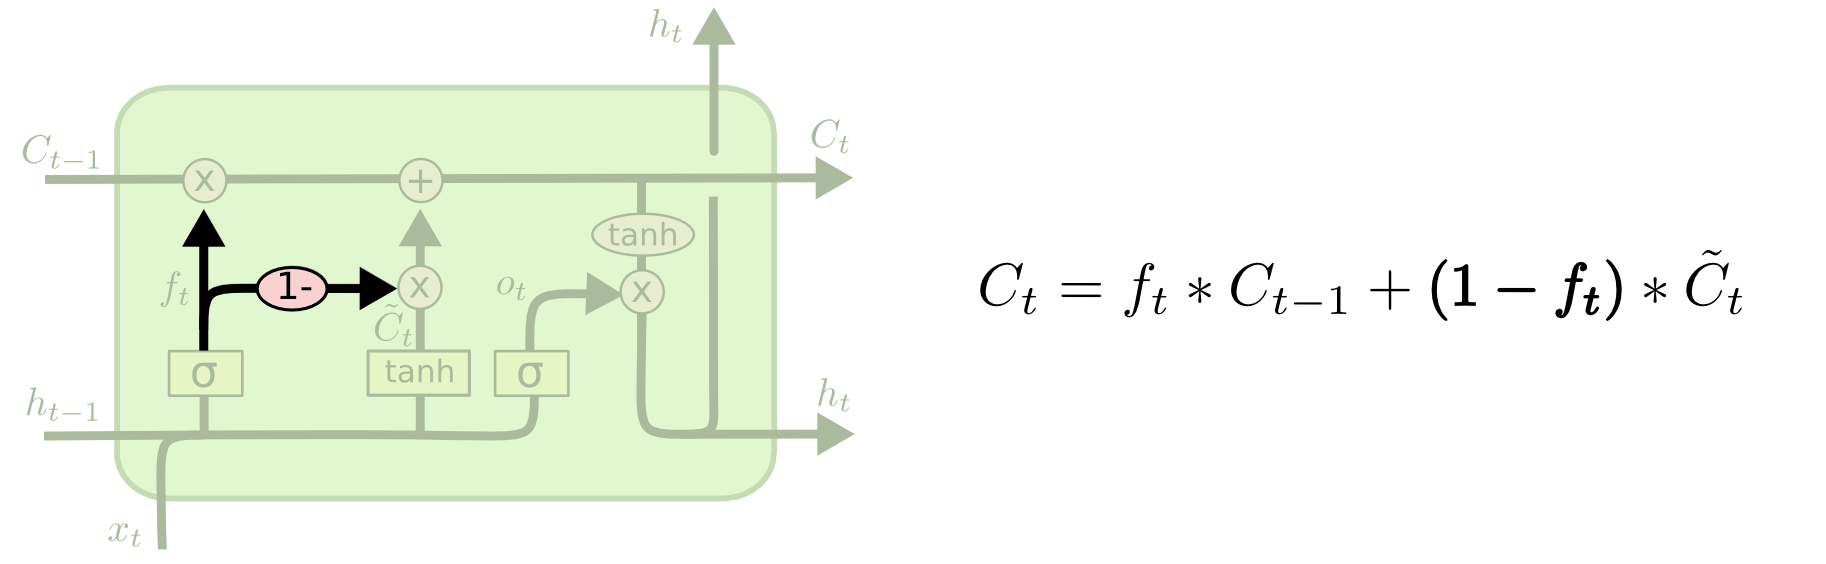
\includegraphics[width=0.60\textwidth]{pictures/LSTM3-var-tied.png}
\caption[LSTM tied]{LSTM tied (Quelle: \cite{OlahImg})}
\end{figure}
A slightly more dramatic variation on the LSTM is the Gated Recurrent Unit, or GRU, introduced by Cho, et al. (2014). It combines the forget and input gates into a single "update gate." It also merges the cell state and hidden state, and makes some other changes. The resulting model is simpler than standard LSTM models, and has been growing increasingly popular.
\renewcommand{\figurename}{Abb.}
\begin{figure}[htp]
\centering
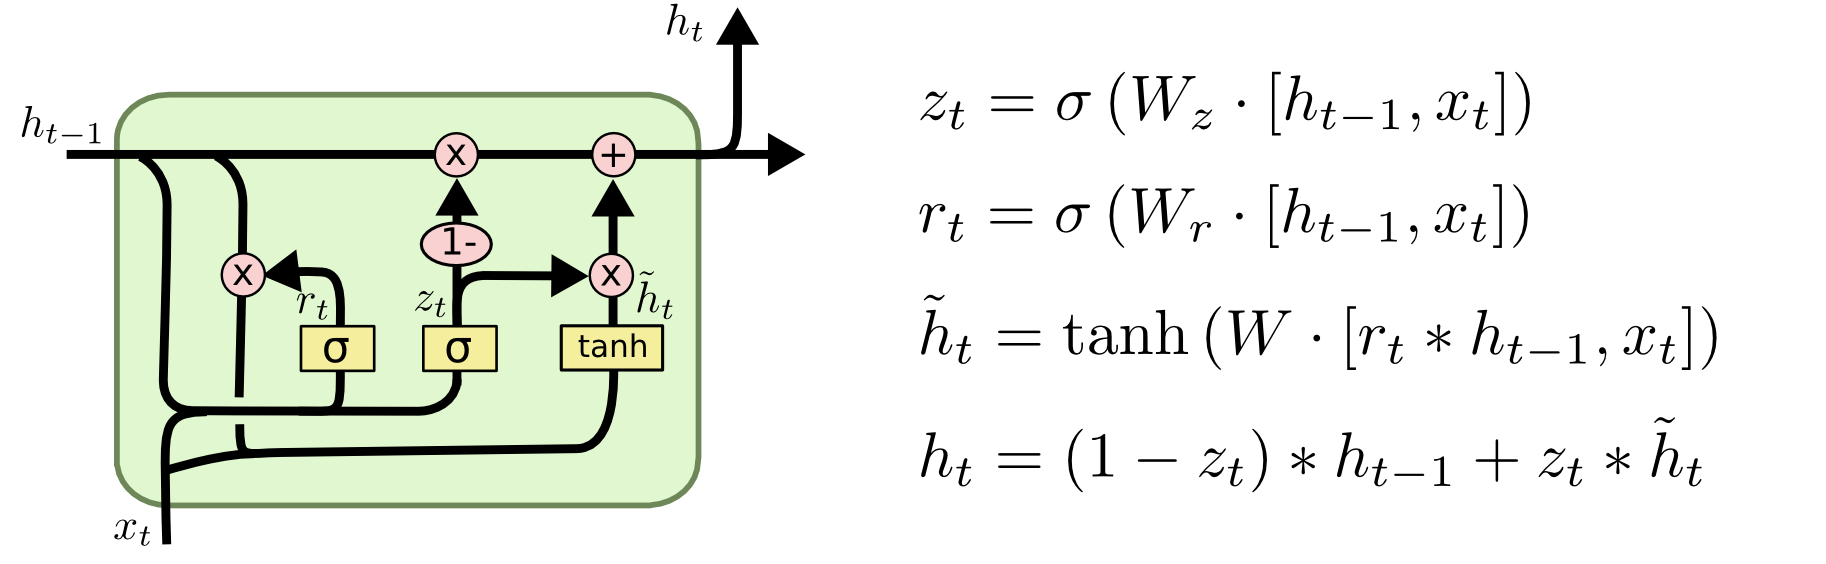
\includegraphics[width=0.60\textwidth]{pictures/LSTM3-var-GRU.png}
\caption[LSTM GRU]{LSTM GRU (Quelle: \cite{OlahImg})} 
\end{figure}
These are only a few of the most notable LSTM variants. There are lots of others, like Depth Gated RNNs by Yao, et al. (2015). There’s also some completely different approach to tackling long-term dependencies, like Clockwork RNNs by Koutnik, et al. (2014).

Which of these variants is best? Do the differences matter? Greff, et al. (2015) do a nice comparison of popular variants, finding that they’re all about the same. Jozefowicz, et al. (2015) tested more than ten thousand RNN architectures, finding some that worked better than LSTMs on certain tasks.


\section{Aktueller Forschungsstand und Problemstellungen (unfinished)}
Charakterisierungen ...

http://deeplearning4j.org/neuralnet-overview\\
As you think about one problem deep learning can solve, ask yourself: What categories do I care about? What information can I act upon? Those outcomes are labels that would be applied to data: spam or not\_spam, good\_guy or bad\_guy, angry\_customer or happy\_customer. Then ask: Do I have the data to accompany those labels? Can I find labeled data, or can I create a labeled dataset (with a service like Mechanical Turk or Crowdflower) that I can use to teach an algorithm the correlation between labels and inputs?

http://deeplearning4j.org/lstm.html
Recurrent nets are a type of artificial neural network designed to recognize patterns in sequences of data, such as text, genomes, handwriting, the spoken word, or numerical times series data emanating from sensors, stock markets and government agencies.

https://colah.github.io/posts/2015-08-Understanding-LSTMs/
In the last few years, there have been incredible success applying RNNs to a variety of problems: speech recognition, language modeling, translation, image captioning… The list goes on. I’ll leave discussion of the amazing feats one can achieve with RNNs to Andrej Karpathy’s excellent blog post, The Unreasonable Effectiveness of Recurrent Neural Networks.
Essential to these successes is the use of "LSTMs," a very special kind of recurrent neural network which works, for many tasks, much much better than the standard version. Almost all exciting results based on recurrent neural networks are achieved with them.

https://colah.github.io/posts/2015-08-Understanding-LSTMs/
LSTMs were a big step in what we can accomplish with RNNs. It’s natural to wonder: is there another big step? A common opinion among researchers is: "Yes! There is a next step and it’s attention!" The idea is to let every step of an RNN pick information to look at from some larger collection of information. For example, if you are using an RNN to create a caption describing an image, it might pick a part of the image to look at for every word it outputs. In fact, Xu, et al. (2015) do exactly this – it might be a fun starting point if you want to explore attention! There’s been a number of really exciting results using attention, and it seems like a lot more are around the corner…
Attention isn’t the only exciting thread in RNN research. For example, Grid LSTMs by Kalchbrenner, et al. (2015) seem extremely promising. Work using RNNs in generative models – such as Gregor, et al. (2015), Chung, et al. (2015), or Bayer \& Osendorfer (2015) – also seems very interesting. The last few years have been an exciting time for recurrent neural networks, and the coming ones promise to only be more so!

http://deeplearning4j.org/lstm.html
In the mid-90s, a variation of recurrent net with so-called Long Short-Term Memory units, or LSTMs, was proposed by the German researchers Sepp Hochreiter and Juergen Schmidhuber as a solution to the vanishing gradient problem.

http://deeplearning4j.org/lstm.html
In the mid-90s, a variation of recurrent net with so-called Long Short-Term Memory units, or LSTMs, was proposed by the German researchers Sepp Hochreiter and Juergen Schmidhuber as a solution to the vanishing gradient problem.
} %% Ende Chapter{RNN und LSTM}